\newpage
\section{Durchführung}

\subsection{Neuronales Netz}
Durch das neuronale Netz sollen digitale Audiodateien in fünf Merkmalsklassen klassifiziert werden. Dabei kann ein Datenpunkt, also eine Audiodatei, mehreren Merkmalsklassen zugehörig sein. Dies wird als ``Multi-Label-Klassifizierung`` bezeichnet \cite{multilabel-classification}. Wird eine Audiodatei (Eingabevektor) zur Klassifizierung in das neuronale Netz eingegeben, erhält man als Ausgabe einen Ausgabevektor von fünf Werten zwischen 0.00 und 1.00, wobei jeder der fünf Werte  die Ähnlichkeit mit einer der fünf Merkmalsklassen repräsentiert (0.00 $\equiv$ keine Ähnlichkeit, 1.00 $\equiv$ Übereinstimmung). Die Merkmalsklassen wurden wie folgt definiert:
    \begin{itemize}
        \item \textbf{bass:} Das Audiosample enthält Töne aus dem tiefen Frequenzspektrum
       	\item \textbf{pitched:} Das Audiosample enthält Töne aus dem hohen Frequenzspektrum
        \item \textbf{melodic:} Das Audiosample enthält melodische Elemente
        \item \textbf{rhythmic:} Das Audiosample enthält rhytmische Elemente
        \item \textbf{sustained:} Das Audiosample enthält ``flächige`` Elemente, also ``langgezogene`` Töne
    \end{itemize}

Dieses neuronale Netz wird mit selbst generierten Trainingsdaten trainiert und anschließend als fertiges Modell mittels dem STM32 proprietären Tool ``STM32Cube.AI`` in C-Code umgewandelt. Damit kann das neuronale Netz im eigenen Code als normale C-Funktion verwendet werden, mit dem Eingabevektor (Audiodaten) als Funktionsparameter und dem Ausgabevektor (Klassifikationsergebnis) als Rückgabewert. \cite{stm32-cube-ai-documentation}

\begin{wrapfigure}{r}{0.4\textwidth}
    \centering
    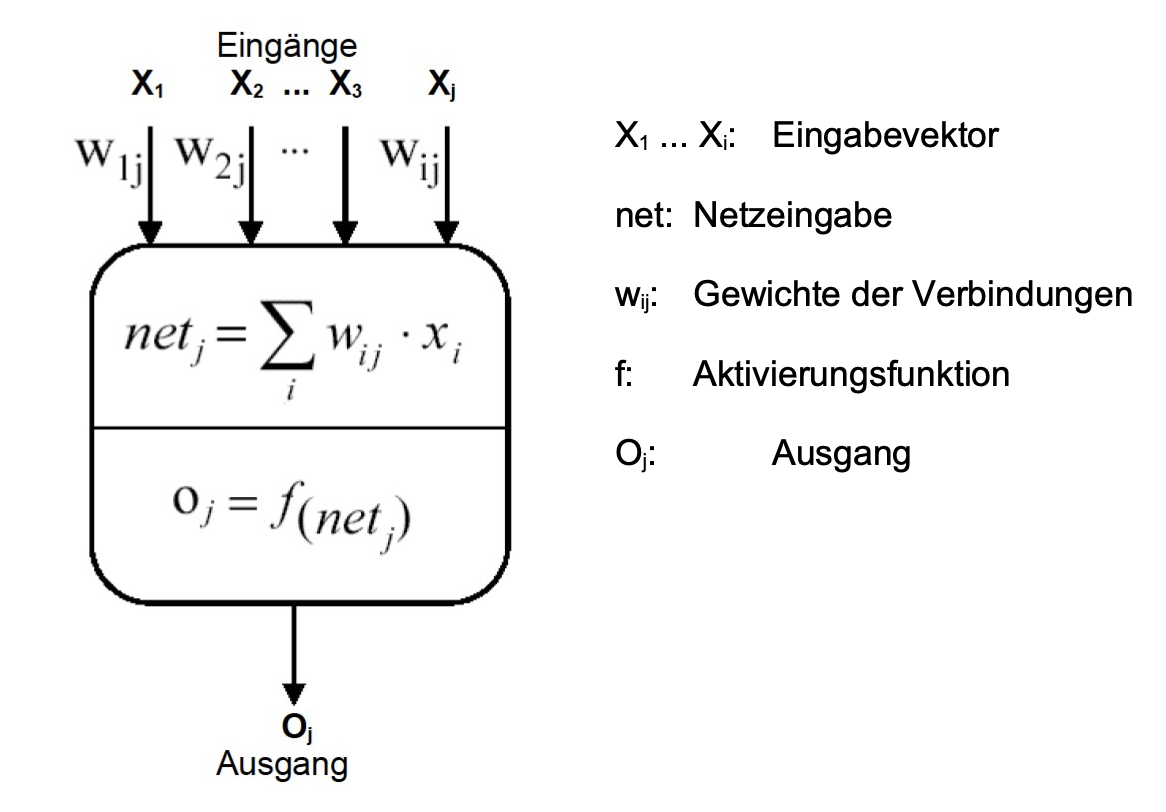
\includegraphics[width=0.4\textwidth]{images/08_durchfuehrung/neuron-aufbau.png}
    \caption{Aufbau des künstlichen Neurons. Quelle: Thieling, Lothar: “Neuronale Netze (Vorlesungsskript ML)”, Kapitel F, Seite 6.}
    \label{fig:img-aufbau-neuron}
\end{wrapfigure}

Die Umwandlung in C-Code ist mögich, da ein Neuron, wie in \textbf{\autoref{fig:img-aufbau-neuron}} dargestellt, aus aus mehreren Gewichten (\textit{W\textsubscript{x}}) in Form eines Vektors besteht, der mit dem Eingabevektor (\textit{X\textsubscript{n}}) des Neurons multipliziert wird. Beide Vektoren sind Fließkommazahlen. Anschließend werden diese Produkte aufaddiert und als Eingabewert einer mathematischen Funktion, der sog. ``Aktivierungsfunktion`` (\textit{f}) verwendet. Der Ausgabewert dieser Funktion ist die Ausgabe des Neurons. \cite{neural-network-basics}

Bei einem neuronalen Netz werden die Neuronen in Schichten hinterheinander angeordnet, die Neuronen der benachbarten Schichten werden vereinfacht gesagt miteinander verbunden, also die Eingabe des einen Neurons bildet eine der Eingaben des nachfolgenden Neurons. \cite{neural-network-basics}

Der ressourcenintensive Teil des Umgangs mit neuronalen Netzen ist das Training, also der Anpassung der Gewichtswerte bis das Neuronale Netz akzeptable Ausgabewerte liefert \cite{neural-network-basics}. Bei diesem Prozess müssen vergleichsweise sehr viele Berechnungen durchgeführt werden. Aus diesem Grund wird das Neuronale Netz zuerst trainiert und erst dann als fertiges Modell in C-Code ungewandelt und auf dem STM32 Microcontroller betrieben. 
Dass das Neuronale Netz fortlaufend durch Benutzerinteraktion weiter trainiert wird, ist nicht vorgesehen.


\subsubsection{Ansatz für die Klassizierung von Audiodaten}
Die Audiodateien liegen als WAVE-Dateien (Dateiendung .wav) vor. Diese enthalten in der Regel pulsweitenmodulierte (PCM) Audiodaten \cite{wav-contains-pcm-data}. Da die Daten nicht komprimiert sind, gehören sie in der Audio- und Musikindustrie zu den gängigsten Dateiformaten \cite{wav-popular-file-format-music-industry}. Eine typische Samplerate für WAVE-Dateien beträgt 44,1 kHz, also 44.100 Samples pro Sekunde, wobei ein Sample in der WAVE-Datei ein quantisierter Amplitudenwert zu einem bestimmten Zeitpunkt ist \cite{wav-pcm-data}. Plottet man dies als Graph, könnte ein Audiosignal wie in \textbf{\autoref{fig:img-pcm-graph}} aussehen.


\begin{figure}[h!]
\centering
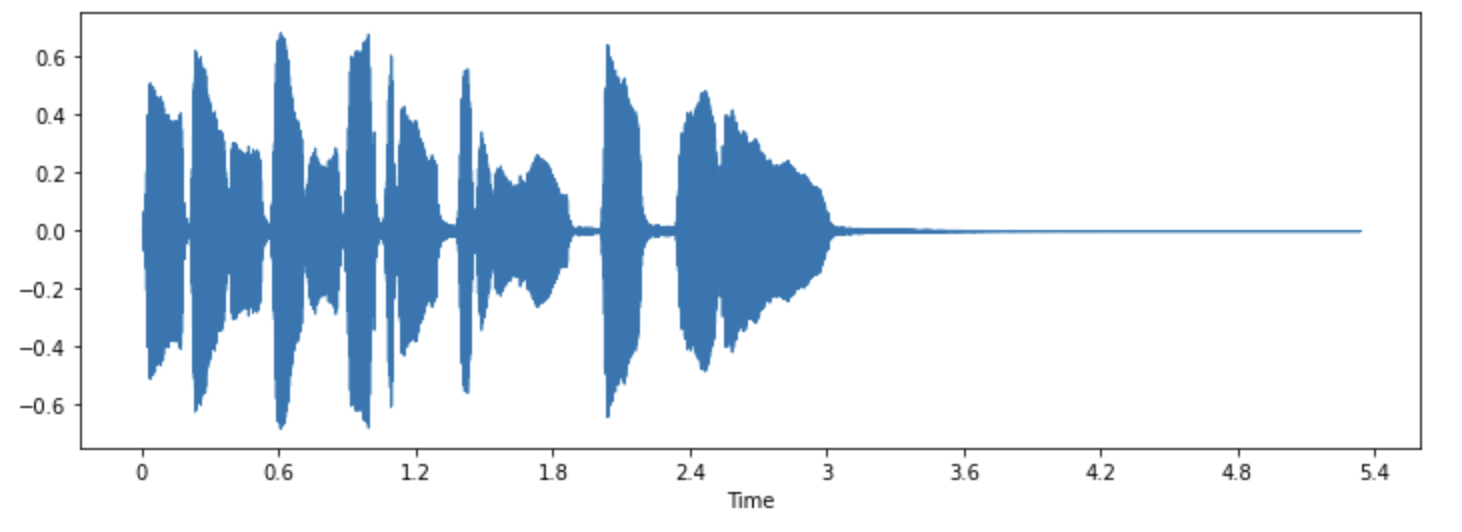
\includegraphics[width=0.4\textwidth]{images/08_durchfuehrung/waveform_plot.png}
\caption{Darstellung eines PCM Audiosignals, Quelle:  https://huggingface.co/learn/audio-course/chapter1/audio\_data TODO }
\label{fig:img-pcm-graph}
\end{figure}

Diese Daten direkt durch ein neuronales Netz klassifizieren zu lassen, ist aus verschiedenen Gründen wenig praktikabel. Die zwei Hauptgründe sind die Merkmalsextraktion und die Größe des Eingabevektors. Letzterer Punkt würde dazu führen, dass selbst bei einer Samplerate von 16 kHz der Eingabevektor 16.000 Werte umfasst. Ein Downsampling auf eine deutlich geringere Zahl, z.B. 1000, ist aufgrund des Shannon-Nyquist-Theorems nicht praktikabel, da dieses besagt, dass die Samplerate mindestens doppelt so hoch sein muss wie die höchste Frequenz \cite{nyquist}. Damit läge der klassifizierbare Frequenzbereich nur im Bereich von \textit{0 Hz} bis maximal \textit{1000 / 2 = 500 Hz}.

Deutlich geeigneter ist es, die Daten als Spektrogramm (Amplitude der verschiedenen Frequenzen eines Signals über die Zeit) wie in \textbf{\autoref{fig:img-spectrogram}} darzustellen und mit einem Convolutional Neural Network (CNN) zu klassifizieren. CNNs werden in erster Linie zur Klassifizierung von Bildern eingesetzt. Die wesentliche Idee ist, dass das neuronale Netz dann nicht nur klassifiziert, sondern auch die Bildvorverarbeitung und die Merkmalsextraktion übernimmt \cite{how-cnn-work}. Da die Audiodateien für das menschliche Gehör klassifiziert werden, sind Mel-Spektrogramme besonders geeignet. Sie basieren auf der Mel-Skala, die das menschliche Gehör nachahmt. Die Mel-Skala ist eine nichtlineare Skala der Frequenzen, die mehr Gewicht auf tiefere Frequenzen legt \cite{mel-spectrogram}.

\begin{figure}[h!]
\centering
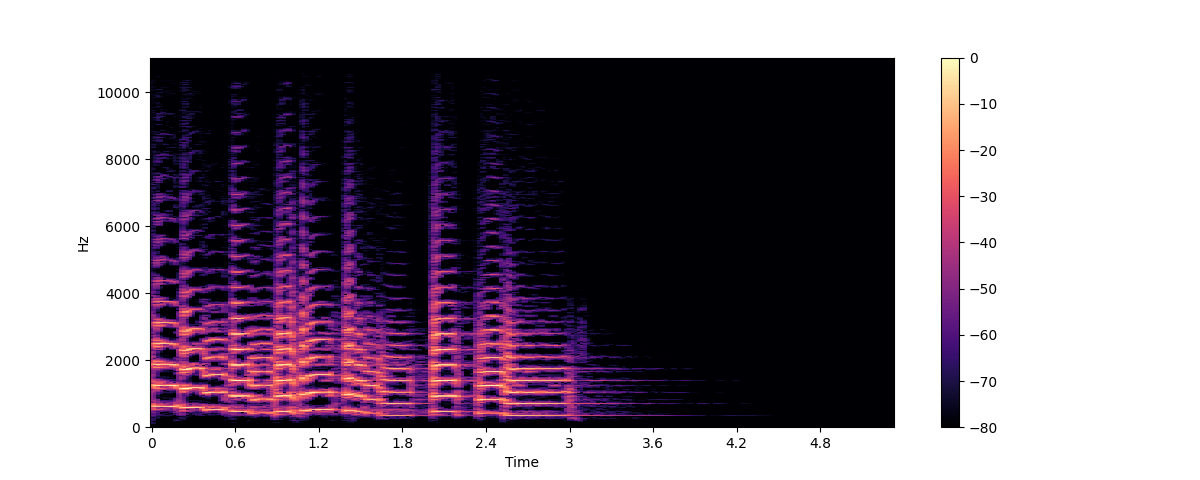
\includegraphics[width=0.75\textwidth]{images/08_durchfuehrung/spectrogram_plot.png}
\caption{Darstellung eines Audiosignals als Spektrogramm, Quelle:  https://huggingface.co/learn/audio-course/chapter1/audio\_data TODO }
\label{fig:img-spectrogram}
\end{figure}

Der limitierende Faktor beim Einsatz eines CNN auf einem Microcontroller sind die Hardwareressourcen, also in erster Linie Flash-Speicher und RAM.

Aufgrund der fehlenden Erfahrungswerte der Teammitglieder mit der möglichen Komplexität von neuronalen Netzen, die mit den Hardwareressourcen eines Microcontrollers betrieben werden können, wird sich auf ein Beispielprojekt von STMicroelectornics gestützt. Dieses heißt ``Acoustic Scene Classification`` \cite{stm-asc}\cite{stm-asc-2}. Basis ist die Klassifizierung von 30x32 px großen Mel-Spektrogrammen mit einem zwei Schichten CNN, die einen Eingabevektor von \textit{32 x 30 = 960} Werten ergeben. 

Sowohl die Dimensionierung der Spektrogramme, als auch die Topologie des Neuronalen Netzes, die Anzahl der Neuronen je Schicht und Elemente der Datenvorverarbeitung wurden aus diesem Projekt übernommen. Damit ist sicher gestellt, dass das Neuronale Netz am Ende nicht die Ressourcen des Microcontrollers übersteigt.

\subsubsection{Generieren der Trainingsdaten}
Für das Training des neuronalen Netzes sind Trainingsdaten erforderlich. Diese bestehen aus Eingabedaten, die bereits mit den korrekten Klassifikationsergebnissen, also Labels, versehen sind.

Da online keine kostenlosen und bereits mit den passenden Labels versehene Datensätze gefunden werden konnten, wurden eigene Daten generiert. Grundlage hierfür bildet eine private Audiosample-Bibliothek. Ein eigens entwickeltes Python-Skript ermöglicht es, Audiosamples auszuwählen, abzuspielen und zeiteffizient zu labeln.

Für jedes manuell gelabelte Audiosample wird eine eindeutige Identifikationsnummer (UID) generiert. Die zugehörigen Labels werden in einer CSV-Datei gespeichert. Ein Beispiel für einen solchen Datensatz zeigt \textbf{\autoref{tab:audiodaten}}. Außerdem wird eine Kopie des Audiosamples unter dem Namen der UID im Ausgabeordner des Skripts abgelegt. Diese Dateien werden später vom Jupyter-Notebook für das Training verwendet.

\begin{table}[h!]
\centering
\begin{tabular}{|m{2.8cm}|m{4.5cm}|m{0.8cm}|m{1.2cm}|m{1.5cm}|m{1.5cm}|m{1.3cm}|}
\hline
\textbf{UID} & \textbf{File} & \textbf{bass} & \textbf{pitched} & \textbf{sustained} & \textbf{rhythmic} & \textbf{melodic} \\ \hline
ecfad96b740844c3
9c96127279f22cf6 &  BD 606 Long MPC60 01.wav & 1 & 0 & 0 & 1 & 0 \\ \hline
\end{tabular}
\caption{Beispielhafter Datensatz eines Audiosamples}
\label{tab:audiodaten}
\end{table}

Bei der Auswahl der Audiosamples wurde darauf geachtet, dass die Daten annähernd gleich verteilt sind, um eine ausgewogene Trainingsbasis zu schaffen. Ein Ungleichgewicht in den Daten kann sich negativ auf das Training und die Klassifikationsergebnisse auswirken. Überrepräsentierte Merkmale könnten die Klassifikationsschwellenwerte beeinflussen, sodass die häufiger vorkommenden Klassen später bevorzugt erkannt werden. Wie in \textbf{\autoref{tab:img-class-spread-graph}} zu sehen, ist die Gleichverteilung jedoch zugegebenermaßen nur mäßig gelungen und hätte einen größeren Zeitaufwand erfordert.

\begin{figure}[h!]
\centering
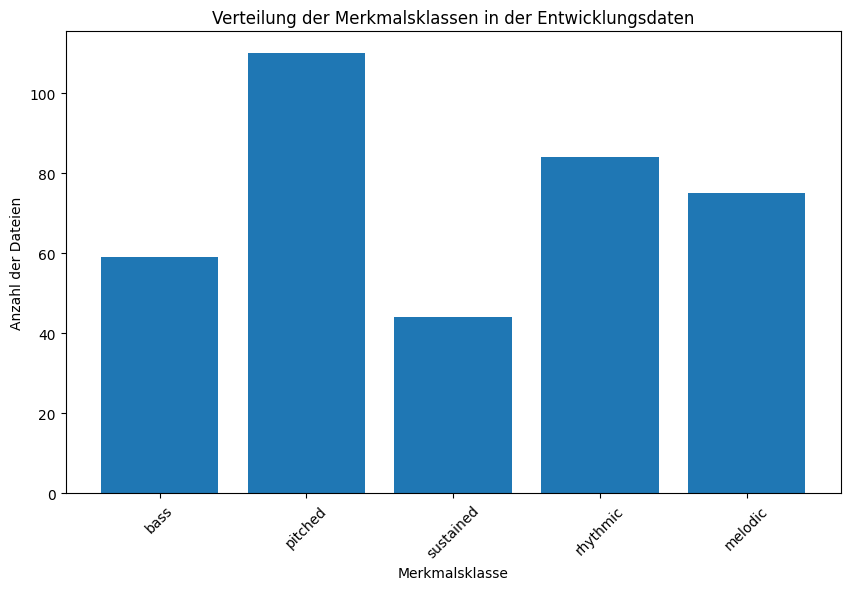
\includegraphics[width=0.75\textwidth]{images/08_durchfuehrung/class_spread_plot.png}
\caption{Repräsentation der verschiedenen Merkmalsklassen in den Entwicklungsdaten}
\label{fig:img-class-spread-graph}
\end{figure}

Zudem wurde sichergestellt, dass der Variationsbereich jeder Klasse möglichst umfassend abgedeckt ist. Dies umfasst sowohl reine Formen jeder Klasse – beispielsweise bei „pitched“ Audiosamples ausschließlich mit Tönen aus dem hohen Frequenzbereich – als auch Mischformen, die Merkmale mehrerer Klassen kombinieren.


\subsubsection{Datenvorverarbeitung}

\subsubsection{Training des Neuronalen Netzes}

\subsubsection{Betrieb des Neuronalen Netzes auf dem STM32 Microcontroller}

\begin{itemize}
    \item Implementierung der Komponenten:
    \begin{itemize}
        \item Ansätze/Methoden: Beschreibung der Ansätze und Methoden für jedes Teilprojekt
        \item Verwendete Komponenten: Detaillierte Beschreibung der verwendeten Komponenten
        \item Erkenntnisse während der Implementierung: Erfahrungen und Änderungen während der Implementierung und Begründung für Alternativen
    \end{itemize}
    \item Integration der Komponenten: Integration der Komponenten in das Gesamtsystem (aus zeitlichen Gründen nicht erfolgt)
\end{itemize}